\chapter{Uvod}


Ovaj završni rad dio je doktorskog rada koji se bavi analizom hrkanja. Za provođenje istraživanja potrebno je sakupiti bazu zvučnih zapisa nad kojima će se provoditi obrada. Budući da se istraživanje i snimanje provode u bolnici, gdje postoje ograničenja nad uređajima koji nadziru i snimaju pacijente, potrebno je razviti neinvazivno softversko i hardversko rješenje koje će snimati i slati podatke na udaljenu lokaciju. Kao uređaj za snimanje zvuka odabran je mikrokontroler STM32WB5M koji će snimati hrkanje i slati snimljeni zvučni zapis Bluetoothom na računalo.  

U okviru ovog završnog rada razvijena je programska potpora za mikrokontroler STM32WB5M te je uspostavljeno BLE komunikacijsko sučelje između razvojnog sustava i osobnog računala s operacijskim sustavom Linux. Sučeljem se prenosi zvučni signal sniman MEMS mikrofonom s mikrokontrolera na računalo. Također je i razvijeno korisničko sučelje za pokretanje komunikacije, prijem i pohranu signala. Blok shema sustava prikazana je na Slici 1.1. 

\begin{figure}[ht]
	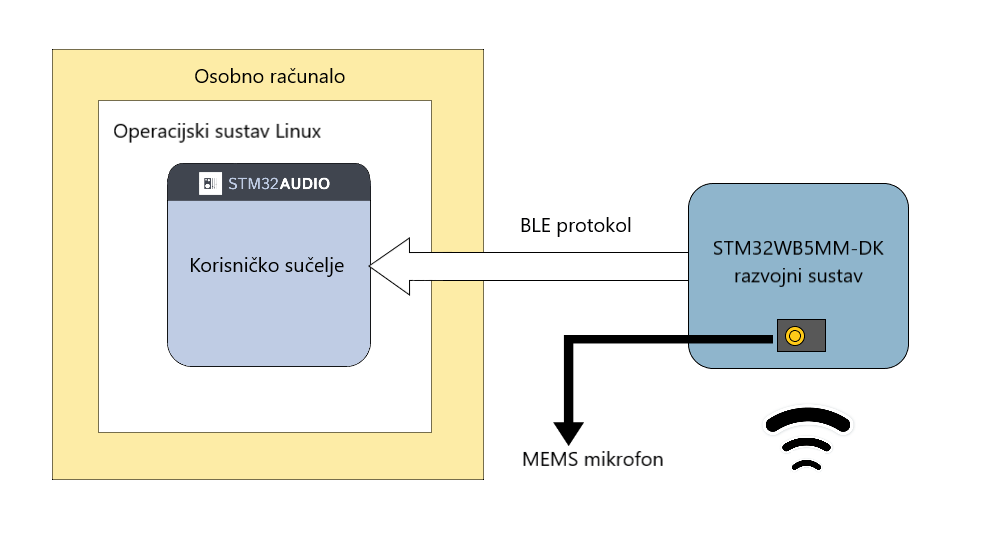
\includegraphics[width=\linewidth]{imgs/shema}
	\caption{Blok shema sustava}
	 \label{fig:shema}
\end{figure}

\eject